\subsection{Level 1.2: 住宅価格を推定するモデルについて}
\subsubsection{課題説明}
Housing Data Set\cite{housingdata}
におけるRM(平均部屋数)からMEDV(平均価格)を推定するた
めのモデルについて検討した。

\subsubsection{モデル}
自分たちの班では一次関数をグラフの中に引くという案が出た.点が密集している部分を通るように,一次関数を引くという方法である.


\subsubsection{モデルへの入力}
平均価格の数値をこの一次関数に入力.
\subsubsection{モデルにおける処理内容}
一次関数は入力された数値に比例する値を出力する.
\subsubsection{モデルの出力}
出力された値というのは,平均価格に対する部屋数を表している.
\subsubsection{問題点}
この方法はある程度の比較された値を求めることが可能であるが,その一次関数から著しく離れた値を切り捨てることになるのでそのあたりの数値に関して信憑性が保てないという問題点がある.

% (補足:PDF図を挿入する例)

% \begin{figure}[h]
%  \begin{center}
%   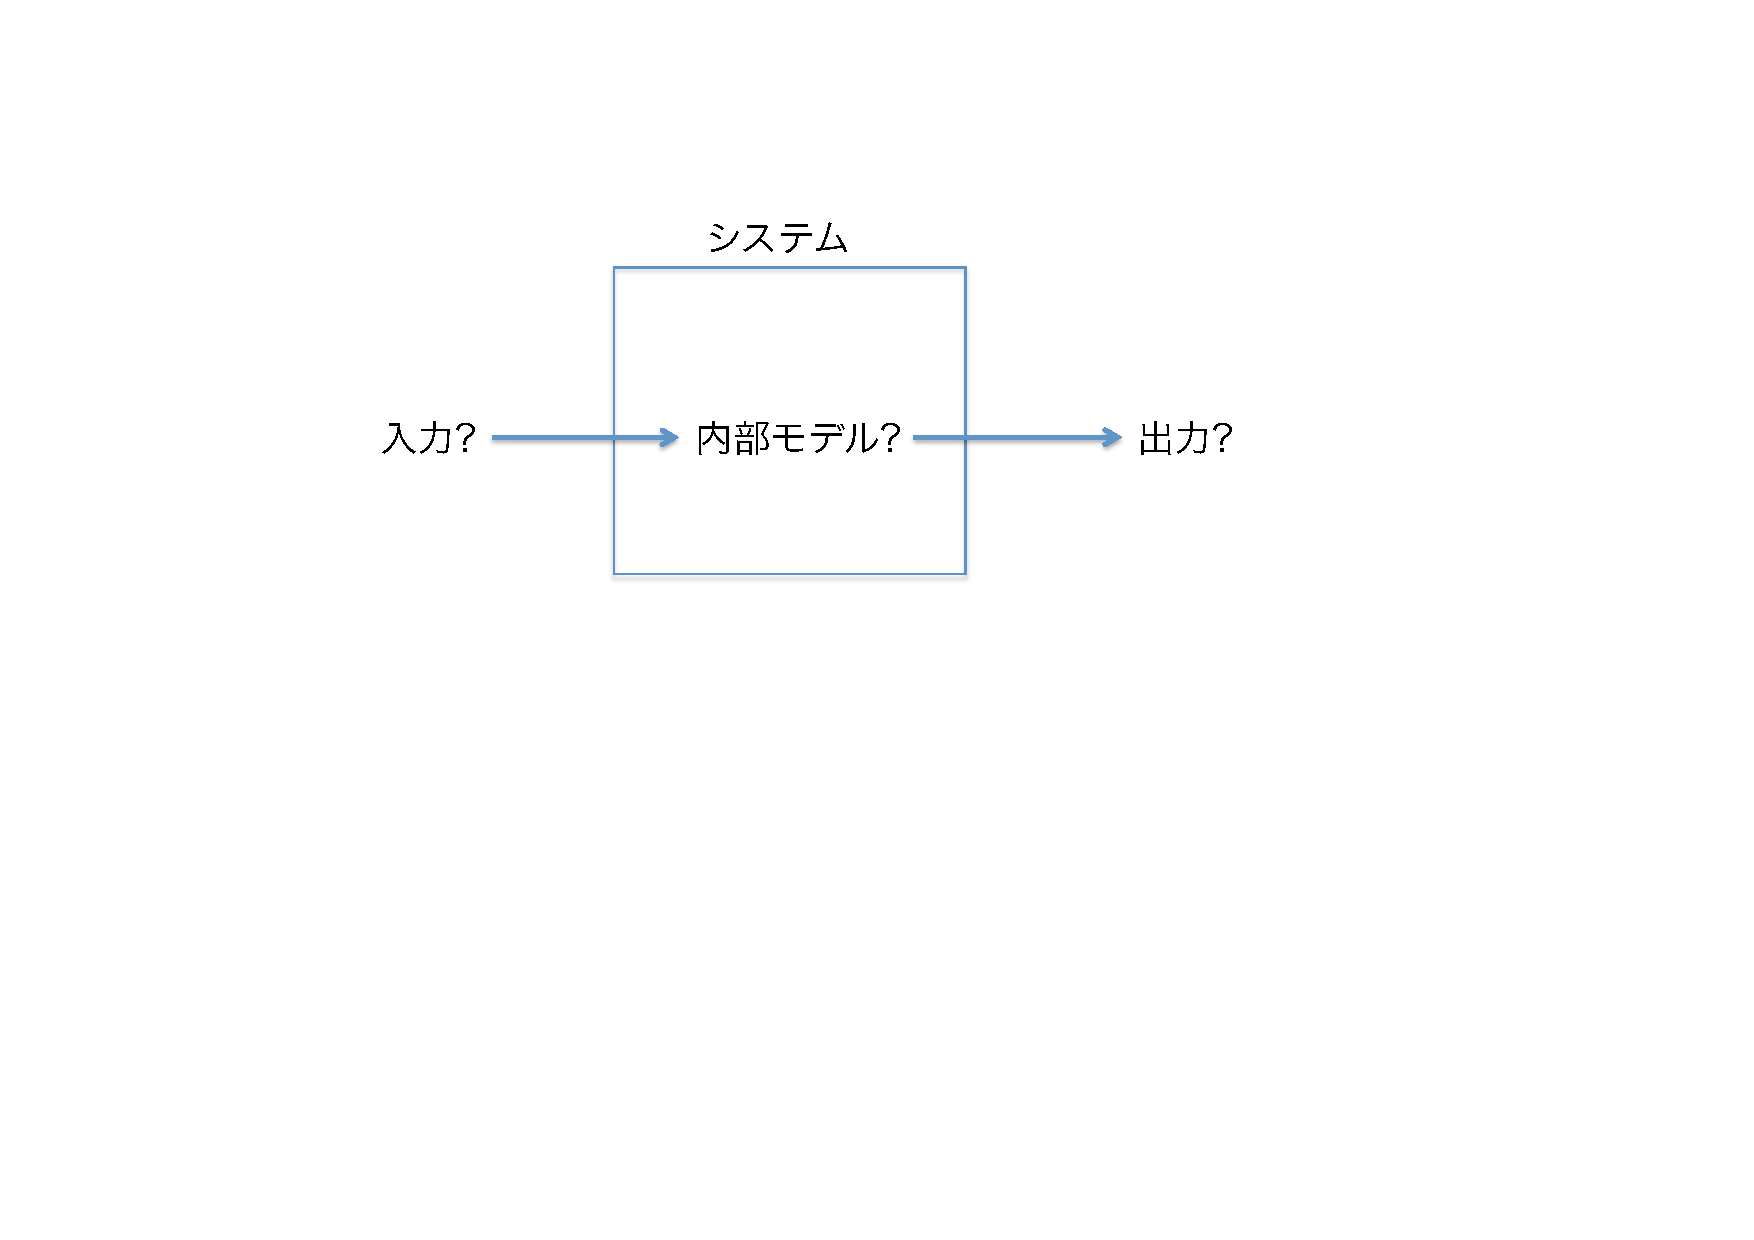
\includegraphics[width=8.0cm]{figs/system-image.pdf}
%   \caption{入出力と内部モデルのイメージ図}
%  \end{center}
% \end{figure}

